
% Subsection '2a'
% Tier 0 and Tier 1's
%
%\subsection{Deployment at the Tier-0 and Tier-1 sites}
%Efforts were made to investigate whether the WLCG software packages could be enabled to run in a dual-stack environment or even become protocol agnostic. The first software packages that were examined were data transfer software packages like FTS and SRM. After the examination some software packages were replaced like AFS with EOS, or CASTOR with DPM. Today the storage environment is dual/stack ready and at CERN the Tier-0 is IPv6 and IPv4 dual-stack enabled. The Tier-1 sites: CA-Triumf, DE-KIT, ES-PIC, FR-CCIN2P3, IT-INFN-CNAF, NDGF, NL-T1 (SARA-Matrix and NIKHEF), RRC-JINR-T1, TW-ASGC, UK-T1-RAL, US-T1-BNL, US-T1-FNAL are dual-stack deployed as shown in the following figure. ~\ref{fig:t1ds}.
%\begin{figure}[b]
%\centering
%\includegraphics[width=13cm]{Tier-1-IPv6-dual-stack}
%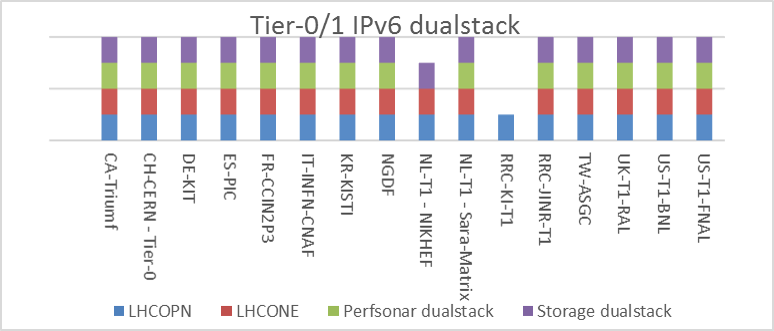
\includegraphics[width=13cm]{hepix-ipv6-tier01-dual-stack.png}
%\includegraphics[width=13cm]{t1ds}
%\caption{Tier-0/1 IPv4/6 dual-stack redyness incl dual-stack perfsonar server deployment}

\subsection{Deployment at Tier-0 and Tier-1's}
After the aforementioned ten years the storage environment is almost completely dual/stack ready and at CERN the Tier-0  and the 14 Tier-1s IPv6 and IPv4 dual-stack is nearly fully enabled. Only the Tier-1 site the Kurchatov Institute in Moscow (part of the Russian Tier-1 Federation) is running on ipv4 only. This enables a total of 95% ipv6 accessible storage of LHC as shown in Figure 1 ~\ref{tab:t12stor}
\begin{table}[h]	
	\centering
	\caption{Fraction of Tier-1 and Tier-2 storage available over IPv6}
	\label{tab:t12stor}
	\begin{tabular}{lccccc}
	\hline
	& ALICE & ATLAS & CMS & LHCb & Global \\\hline
	Tier-1 storage & 78\% & 96\% & 100\% & 94\% & 96\% \\ 
	Tier-2 storage & 86\% & 59\% & 89\% & 75\% & 74\% \\\hline
	\end{tabular}
	\end{table}
The FTS server at FNAL is still running in IPv4 preferred mode. There was a long standing malfunctioned transfer issue to IPv4 only US-Tier-2 sites which is solved now. This last server will get deployed in dual-stack as soon as possible.
